\documentclass[12pt,a4paper]{article}

\usepackage[utf8]{inputenc}
\usepackage[T1]{fontenc}
\usepackage[serbian]{babel}
\usepackage{amsmath}
\usepackage{graphicx}
\usepackage{booktabs}
\usepackage{hyperref}
\usepackage{geometry}
\usepackage{float}
\usepackage{caption}
\usepackage{subcaption}

\geometry{margin=2.5cm}

\title{\textbf{Analiza strukture ličnosti primenom metoda klasterovanja}\\Projekat iz Istraživanja podataka 2 
[R275]}
\author{Ksenija Ivanović 135/2019}
\date{Školska 2025/26 godina}

\begin{document}

\maketitle

\tableofcontents
\newpage

\section{Uvod}

\subsection{Opis problema}

U ovom radu analiziramo podatke prikupljene putem Big Five Personality testa, jednog od najuticajnijih i empirijski najpotvrđenijih modela ličnosti u savremenoj psihologiji. Model opisuje ličnost kroz pet osnovnih dimenzija:

\begin{itemize}
    \item Ekstraverzija (Extraversion)
    \item Neuroticizam (Neuroticism)
    \item Prijatnost (Agreeableness)
    \item Savesnost (Conscientiousness)
    \item Otvorenost ka iskustvu (Openness to Experience)
\end{itemize}

Svaka dimenzija meri se pomoću više tvrdnji koje ispitanici ocenjuju na Likertovoj skali (od 1 do 5). Agregacijom odgovora dobija se numerički skor koji predstavlja izraženost određene osobine kod pojedinca.

Iako se osobine ličnosti tradicionalno posmatraju kao kontinuirane dimenzije, postavlja se pitanje da li se ispitanici mogu prirodno grupisati u određene tipove ličnosti. Drugim rečima, da li u podacima postoji latentna struktura koja ukazuje na postojanje relativno stabilnih grupa pojedinaca sa sličnim profilima osobina?


\begin{figure}[H]
    \centering
    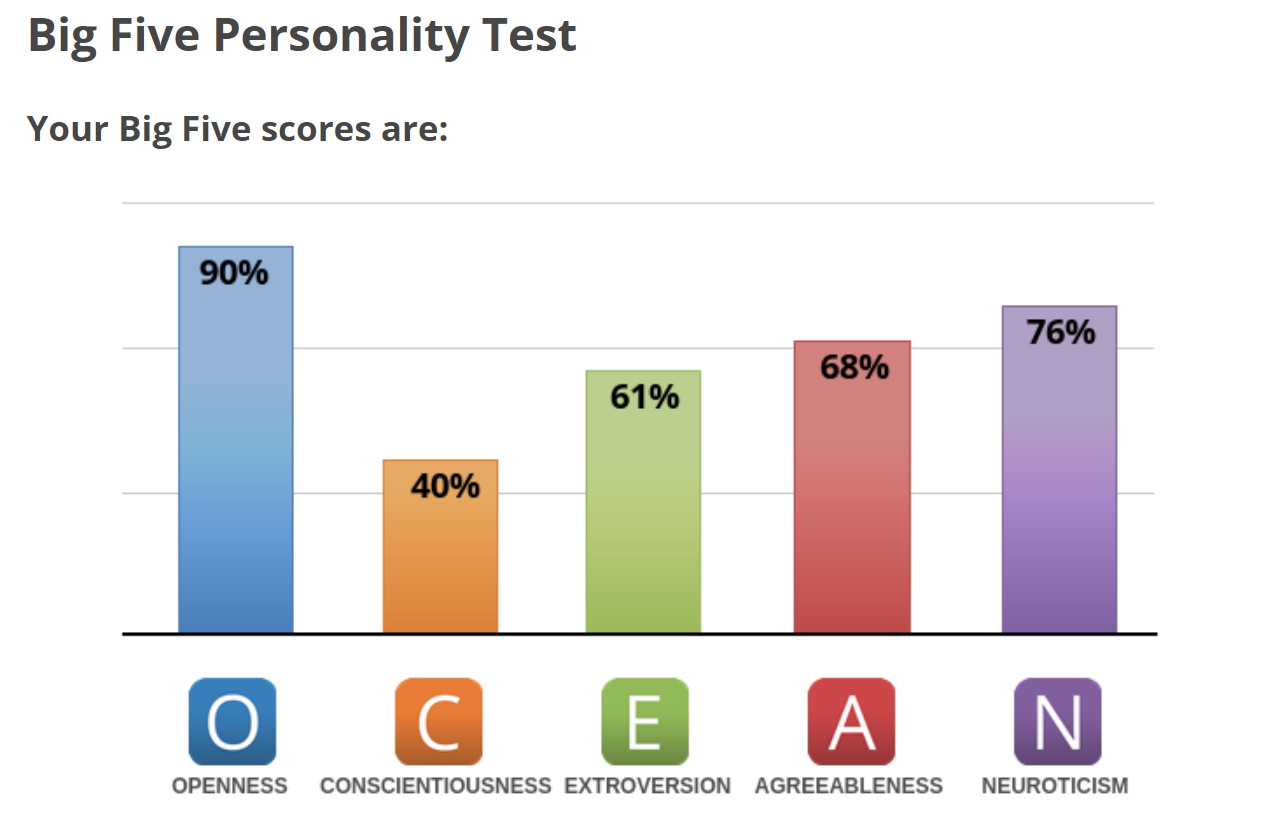
\includegraphics[width=0.7\textwidth]{../slike/bigfive.png}
    \caption{Primer prikaza rezultata Big Five testa}
    \label{fig:big5}
\end{figure}


Ovaj rad ima za cilj da ispita postojanje takve strukture primenom metoda nenadgledanog učenja.

\subsection{Cilj rada}

Cilj rada je da se ispita da li se na osnovu odgovora na Big Five test može identifikovati prirodna segmentacija ispitanika. 

Konkretnije, cilj je:
\begin{itemize}
    \item utvrditi da li postoji jasno izražena klasterska struktura u podacima,
    \item uporediti performanse različitih algoritama klasterovanja,
    \item interpretirati dobijene klastere na osnovu prosečnih vrednosti osobina.
\end{itemize}

\section{Opis podataka}

Podaci koji se analiziraju prikupljeni su u periodu 2016--2018. godine putem interaktivnog onlajn testa ličnosti. Test je konstruisan na osnovu \textit{Big-Five Factor Markers} iz IPIP baze (International Personality Item Pool).

Ispitanici su na početku testa informisani da će njihovi odgovori biti sačuvani i korišćeni u istraživačke svrhe, a na kraju su morali da potvrde saglasnost za korišćenje podataka. U dataset su uključeni isključivo ispitanici koji su dali saglasnost.

\subsection{Struktura upitnika}

Upitnik se sastoji od 50 tvrdnji, po 10 za svaku od pet dimenzija ličnosti:
\begin{itemize}
    \item Ekstraverzija (EXT),
    \item Neuroticizam / Emocionalna stabilnost (EST),
    \item Saradljivost (AGR),
    \item Savesnost (CSN),
    \item Otvorenost ka iskustvu (OPN).
\end{itemize}

Svaka tvrdnja ocenjena je na petostepenoj Likertovoj skali:
\begin{center}
1 = Disagree, \quad 3 = Neutral, \quad 5 = Agree.
\end{center}

Pored samih odgovora, zabeleženo je i vreme odgovaranja na svako pitanje (u milisekundama), što omogućava dodatne analize ponašanja ispitanika tokom popunjavanja testa.

\subsection{Dodatne promenljive}

Dataset sadrži i sledeće tehničke i kontekstualne informacije:

\begin{itemize}
    \item \texttt{dateload} -- vremenska oznaka početka testa,
    \item \texttt{introelapse}, \texttt{testelapse}, \texttt{endelapse} -- vreme provedeno na pojedinim delovima testa,
    \item \texttt{IPC} -- broj zapisa sa iste IP adrese (radi kontrole višestrukih unosa),
    \item \texttt{country} -- zemlja korisnika (određena tehničkim putem),
    \item \texttt{screenw}, \texttt{screenh} -- dimenzije ekrana,
    \item približne geografske koordinate (latitude i longitude), uz napomenu da ove vrednosti nisu precizne.
\end{itemize}

U okviru analize, primarni fokus biće na odgovorima na tvrdnje (50 stavki), dok će dodatne promenljive biti korišćene za filtriranje i inicijalnu obradu podataka (npr. uklanjanje višestrukih unosa korišćenjem promenljive \texttt{IPC}).

\section{Metodologija}

\subsection{Priprema podataka}

Pre primene algoritama klasterovanja izvršeni su sledeći koraci:

\begin{itemize}
    \item Provera i uklanjanje nedostajućih vrednosti.
    \item Eventualna agregacija odgovora po dimenzijama.
    \item Skaliranje numeričkih podataka radi ujednačavanja opsega vrednosti.
\end{itemize}

Skaliranje je posebno važno jer većina algoritama klasterovanja koristi udaljenosti između tačaka, te različiti opsezi varijabli mogu značajno uticati na rezultate.

\subsection{Algoritmi klasterovanja}

U radu su primenjeni sledeći algoritmi:

\begin{itemize}
    \item K-means klasterovanje
    \item Hijerarhijsko (agglomerativno) klasterovanje
    \item DBSCAN
    \item (po potrebi) Spektralno klasterovanje
\end{itemize}

Za algoritme koji zahtevaju unapred definisan broj klastera testirano je više vrednosti parametra $k$, kako bi se procenila stabilnost rezultata.

\subsection{Evaluacija rezultata}

Rezultati klasterovanja upoređeni su korišćenjem sledećih metrika:

\begin{itemize}
    \item Silhouette indeks
    \item Davies--Bouldin indeks
    \item Calinski--Harabasz indeks
\end{itemize}

Na osnovu ovih metrika vršeno je poređenje algoritama i izbor modela koji najbolje opisuje strukturu podataka.

\section{Rezultati}

U ovom poglavlju biće prikazani:

\begin{itemize}
    \item Tabele sa vrednostima evaluacionih metrika.
    \item Vizualizacije klastera pomoću PCA projekcije.
    \item Heatmap prikaz prosečnih vrednosti osobina po klasterima.
\end{itemize}

Na osnovu ovih rezultata izvršiće se interpretacija dobijenih grupa ispitanika.

\section{Diskusija}

U ovom delu rada razmatra se:

\begin{itemize}
    \item Da li postoji jasna prirodna struktura u podacima.
    \item Koliko su klasteri stabilni i interpretabilni.
    \item Ograničenja primenjenog pristupa.
\end{itemize}

\section{Zaključak}

U zaključku će biti sumirani ključni nalazi rada, uz osvrt na pitanje da li Big Five podaci pokazuju postojanje diskretnih tipova ličnosti ili pre predstavljaju kontinuirani spektar osobina.

\end{document}
